\documentclass[aspectratio=169]{beamer}
\usepackage[spanish]{babel}
\renewcommand{\tablename}{Tabla}
\usepackage{ITMOtheme}
\usepackage{csquotes,amsmath}
% Use this package to automatically format references.
\usepackage[backend=biber, style=ieee]{biblatex}
\addbibresource{references.bib}
\renewcommand*{\bibfont}{\scriptsize}
\graphicspath{fig/}
\usepackage{caption,graphicx}
%\usepackage{caption,graphicx,float,csquotes,amsmath,mathptmx,amssymb,amsfonts}
\titlegraphic{
\includegraphics[scale=.3]{itmo/ucvlogo.png}}
\setbeamertemplate{caption}[numbered]

% The fields 'title', 'author', 'subject', 'keywords' are used to generate a PDF document.

% use \title[short title]{full title}
\title[ITMO LaTex]{Control de un motor de paso mediante un controlador comercial.}
%\subtitle[short subtitle]{long subtitle}
\author[LastName F.]{Ricardo Santana}
%\institute[short institute]{long institute}
\where{Caracas}
\date{\today}
\subject{Teoría de la Información.}
\keywords{ITMO University, LaTex teamplate, beamer}


% By default, the title of the presentation (\inserttitle) is written at the bottom of each slide.
% This text can be replaced with something else, for example:
\setfootlinetext{\insertsection}

\begin{document}
% [plain] - modifier to create a blank slide (without bottom bar).
% Ideal for creating the first (title) and last slide with a polygonal background,
% or for transitional slides between chapters or slides with a table of contents.

% \titlepage - command for automatic generation of title slide content.

%portado simple
%\begin{frame}[plain]
%    \titlepage
%    \begin{block}{title}
%        bloque simple (azul).
%    \end{block}
%    \begin{exampleblock}{title}
%        bloque ejemplo (verde).
%    \end{exampleblock}
%    \begin{alertblock}{title}
%        bloque alerta (rojo).
%    \end{alertblock}
%\end{frame}



% You can use custom title, if you want.
% Or you can you modify the .sty file.


\begin{frame}[plain]
	\itmofondo{itmo/fondoelectro.jpg}{
    \vfill
        República Bolivariana de Venezuela \par Universidad Central de Venezuela \par Facultad de Ingeniería\par Escuela de Eléctrica \par Coordinación de Pasantías y Servicio Comunitario.
	\vfill
		
\includegraphics[scale=.3]{itmo/ucvlogo.png}
	\vfill
		\usebeamerfont{title}{  \inserttitle\par}
    \vfill
        %----subtitulo-----
	%\vfill
		\insertauthor ;CI:29571461\par
	\vfill
        Tutor: Ing. Herrera, Alejandro \par
    \vfill
		\insertplace  \;  \insertdate
}
\end{frame}

\AtBeginSection[]
{
    \begin{frame}[plain]
        \frametitle{Contenido}
        \Large
        \tableofcontents[currentsection]
    \end{frame}
}

\section{Objetivos}

\begin{frame}{Objetivos}
    \begin{block}{Objetivo general.}
        \begin{itemize}
            \item Desarrollar una aplicación embebida que controle un motor de paso mediante un controlador comercial, en respuesta a la variación del ángulo de un encoder, mostrando los parámetros clave en una pantalla LCD mediante comunicación I2C o serial.
        \end{itemize}
    \end{block}
    \begin{block}{Objetivos específicos.}
        \begin{itemize}
            \item Estudiar los componentes seleccionados: microcontrolador, controlador del motor, motor de paso, encoder y pantalla LCD.
            \item Implementar la lectura del encoder y su conversión a señales de control para el motor de paso.
            \item Configurar la comunicación entre el microcontrolador y el controlador del motor.
            \item Desarrollar la interfaz de visualización en la pantalla LCD (I2C o serial).
            \item Integración, validación y documentación del sistema.
        \end{itemize}
    \end{block}
\end{frame}

\section{Componentes Indispensables (Hardware)}

\begin{frame}{Componentes}
    \begin{columns}[c]
        \column{0.34\textwidth}{
            \begin{figure}[H]
                \centering
                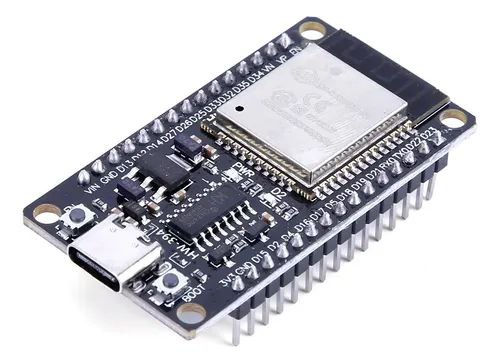
\includegraphics[height=2cm]{fig/esp32.jpg}
                \caption{Microcontrolador: ESP32-WROOM-32.}
            \end{figure}
            \begin{figure}[H]
                \centering
                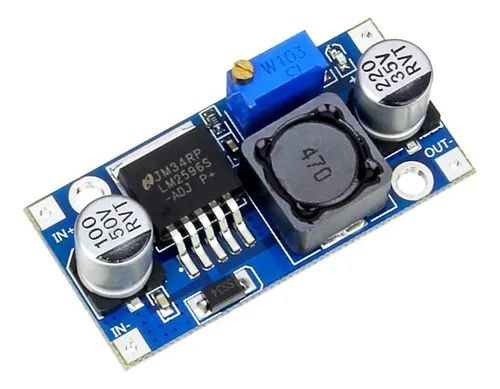
\includegraphics[height=2cm]{fig/convertidor-dc-dc.jpg}
                \caption{Reductor de Voltaje: Módulo LM2596.}
            \end{figure}
        }
        \column{0.34\textwidth}{
            \begin{figure}[H]
                \centering
                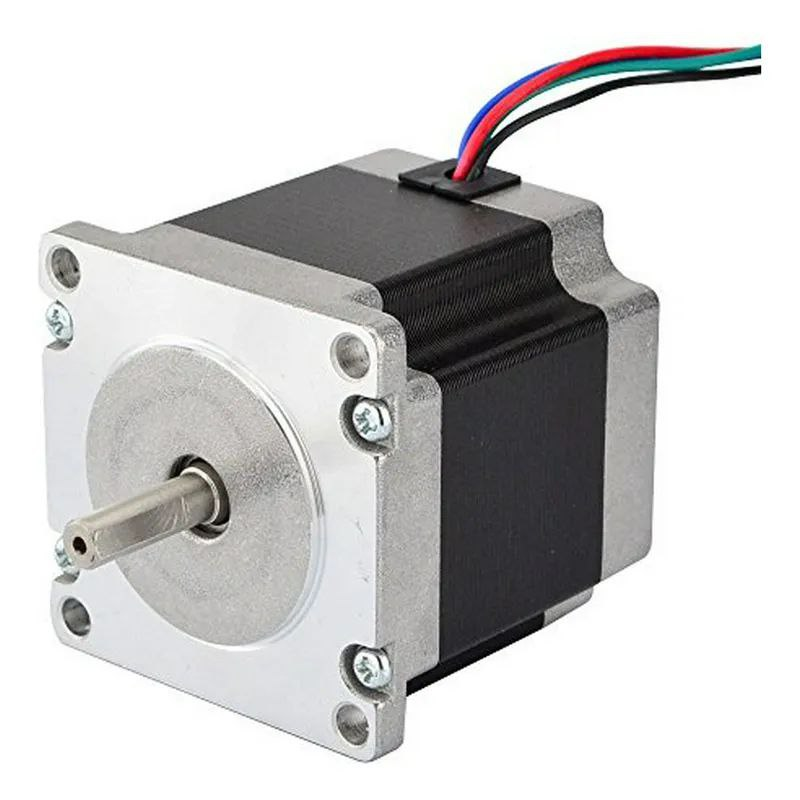
\includegraphics[height=2cm]{fig/stepper-motor.jpg}
                \caption{Motor de Paso: StepperOnline 23HS22-2804S.}
            \end{figure}
            \begin{figure}[H]
                \centering
                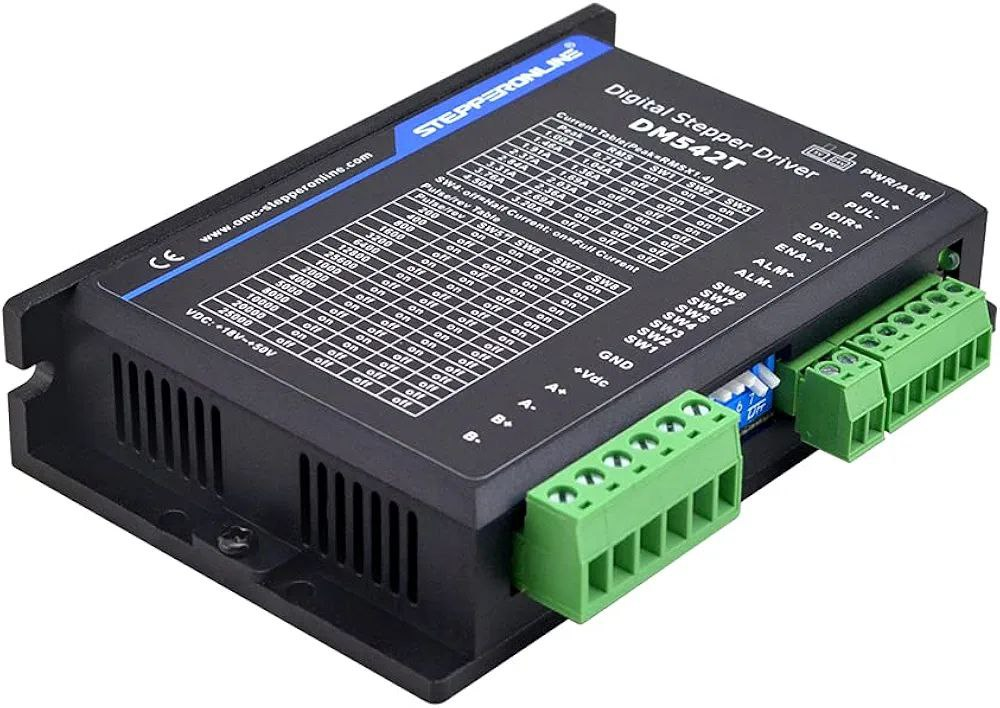
\includegraphics[height=2cm]{fig/driver-motor.jpg}
                \caption{Driver Motor: Digital Stepper Drive DM542T.}
            \end{figure}
        }
        \column{0.34\textwidth}{
            \begin{figure}[H]
                \centering
                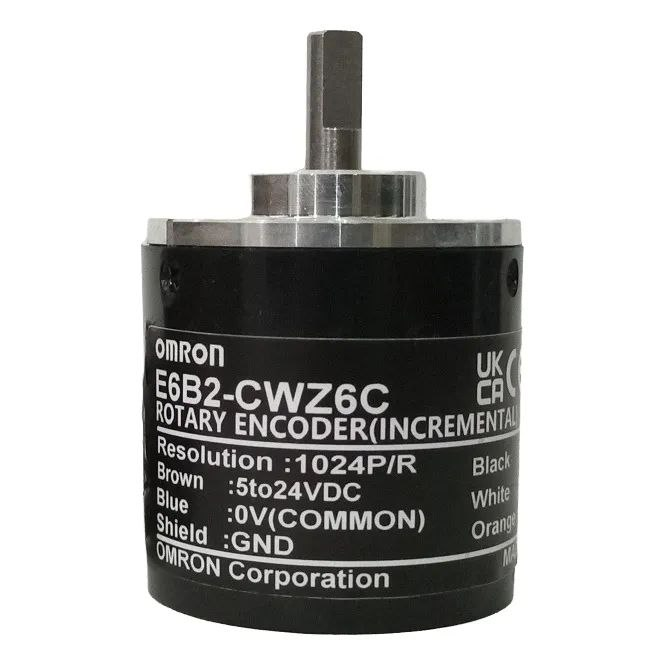
\includegraphics[height=2cm]{fig/encoder.jpg}
                \caption{Encoder Rotativo: Omron E6B2-CWZ6C.}
            \end{figure}
            \begin{figure}[H]
                \centering
                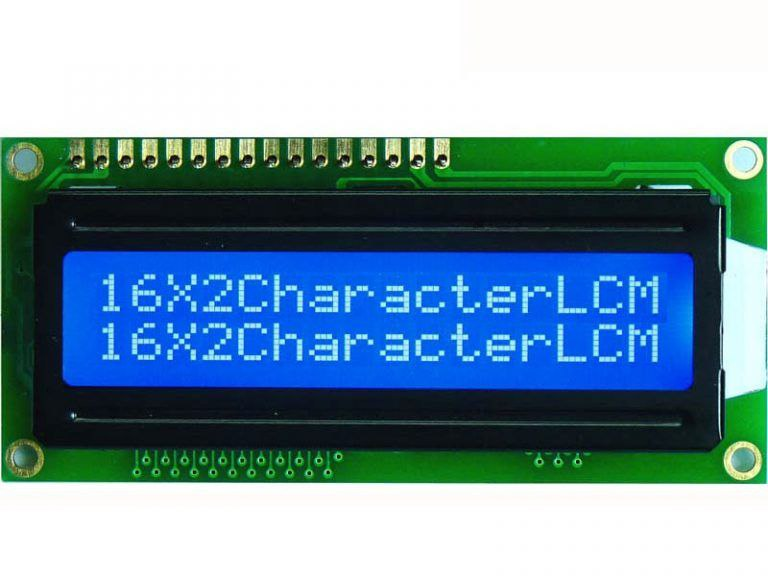
\includegraphics[height=2cm]{fig/pantalla-lcd.jpg}
                \caption{Pantalla LCD WH1602B con adaptador I2C.}
            \end{figure}
        }
    \end{columns}
\end{frame}

\section{Implementación de Encoder.}

\begin{frame}{Prueba de encoder.}
    \begin{columns}[c]
        \column{0.5\textwidth}{
            \begin{figure}[H]
                \centering
                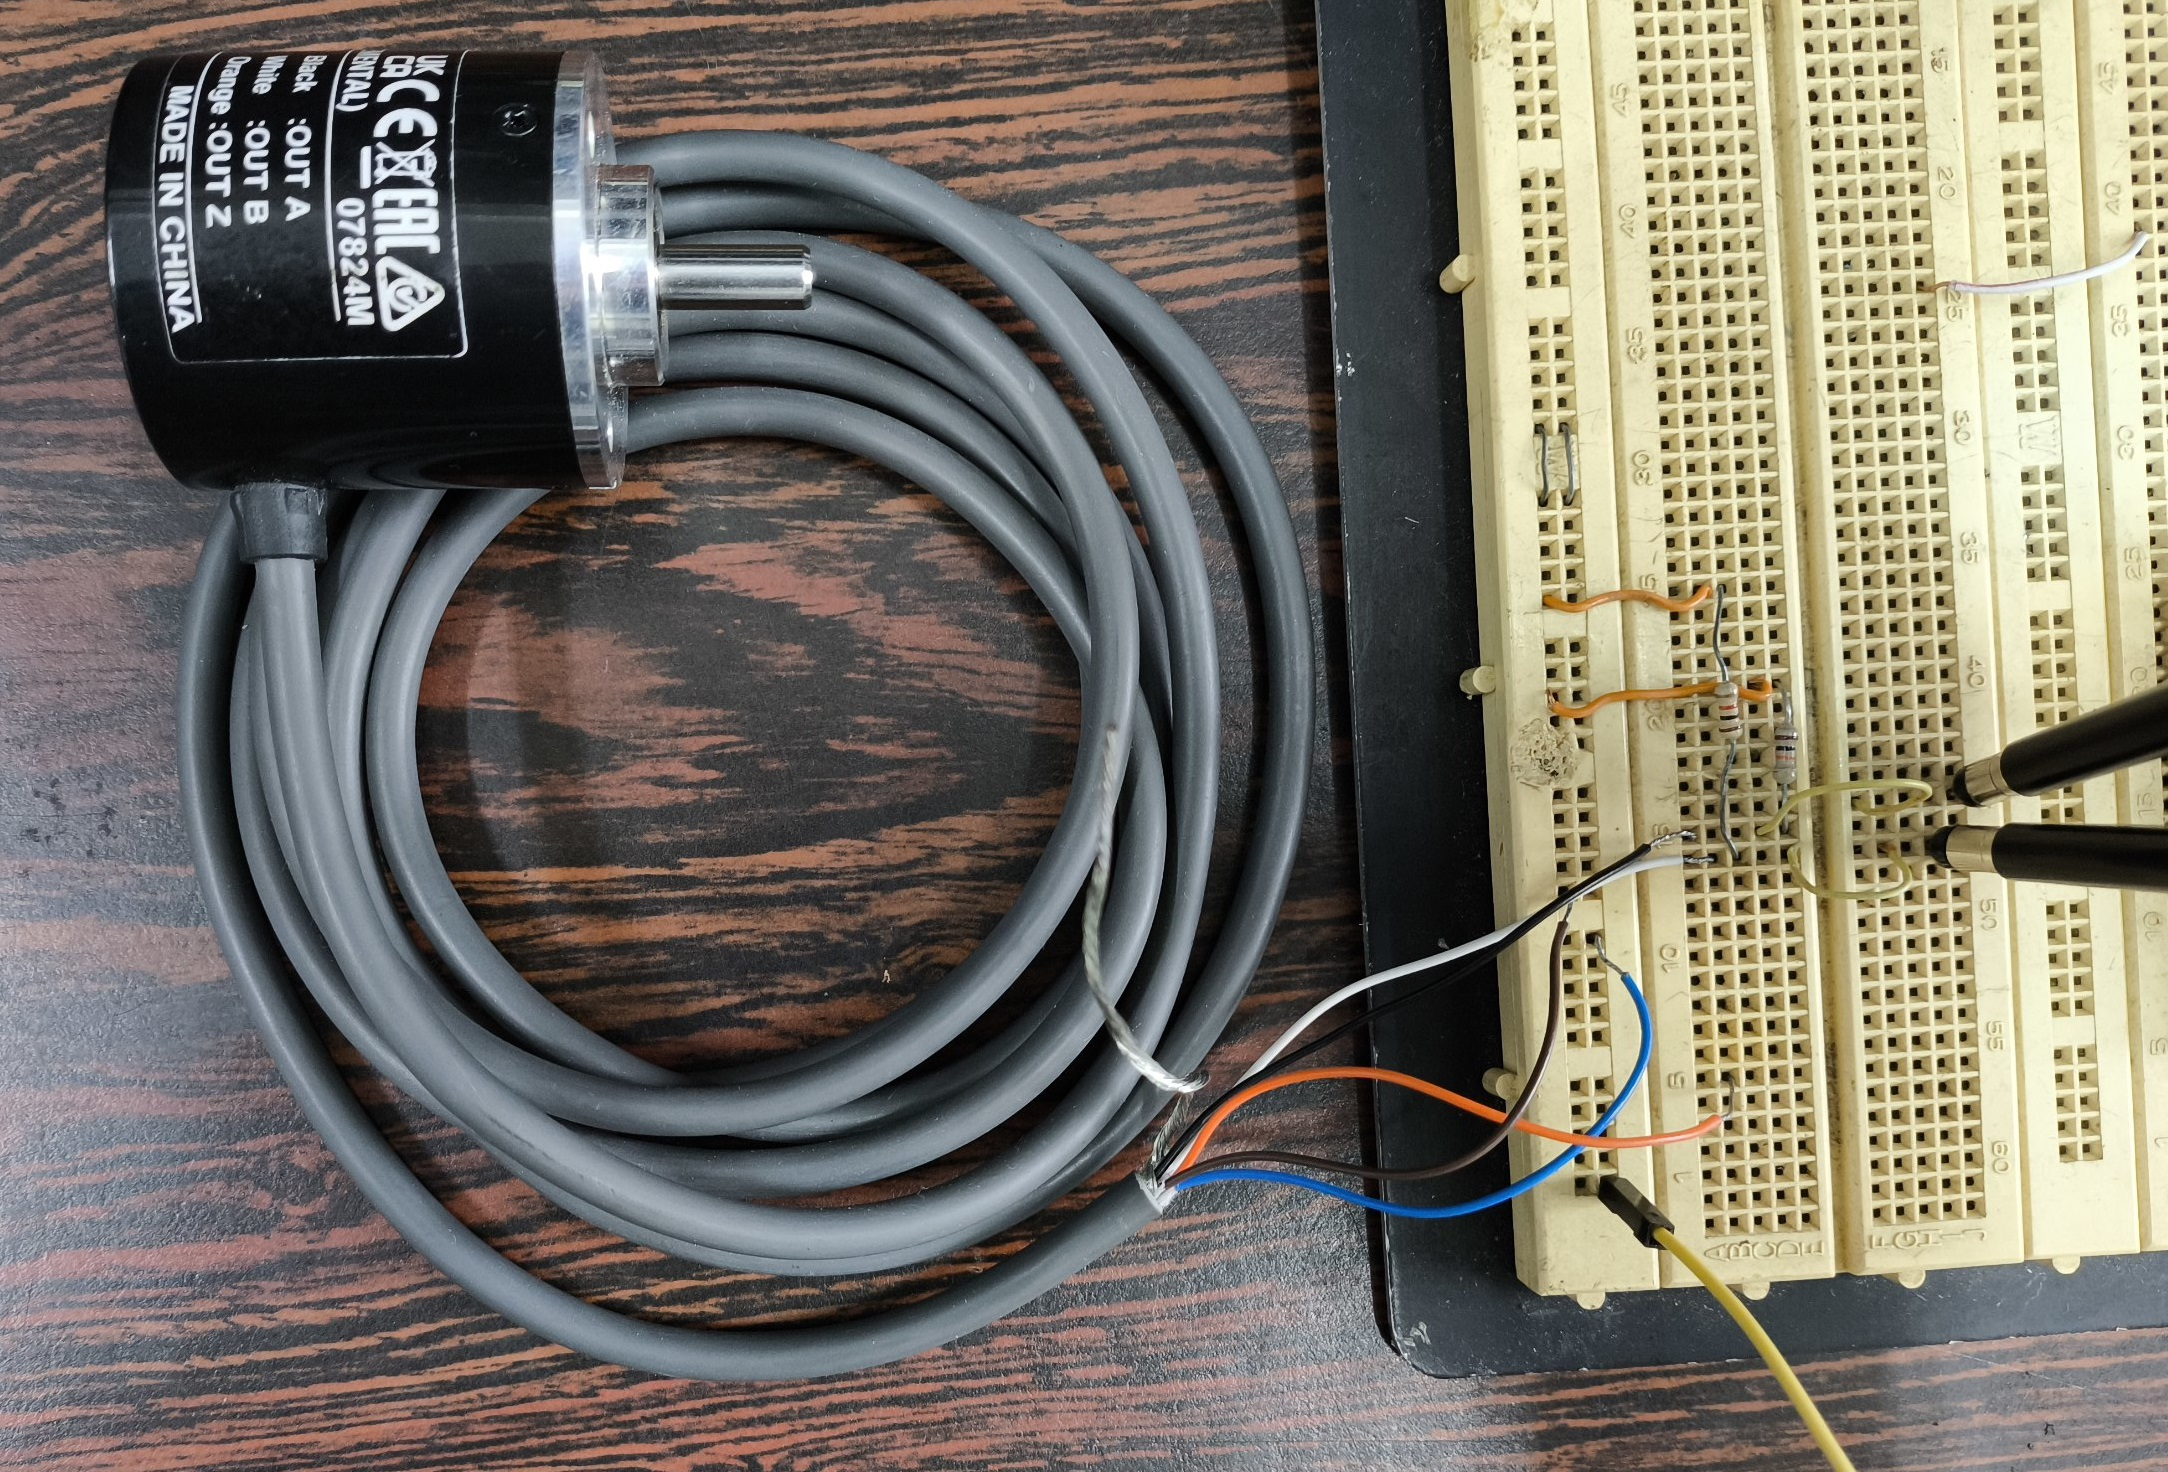
\includegraphics[width=\textwidth]{fig/encoder-prueba.jpg}
                \caption{Montaje para observación y validación del funcionamiento del encoder.}
            \end{figure}
        }
        \column{0.5\textwidth}{
            \begin{figure}[H]
                \centering
                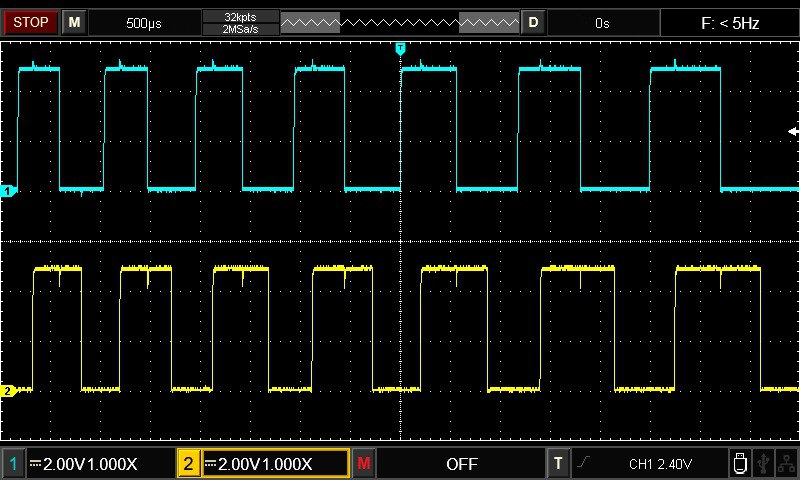
\includegraphics[width=\textwidth]{fig/encoder-senal.jpg}
                \caption{Confirmación de señales recibidas y desfase repectivo de 90°.}
            \end{figure}
        }
    \end{columns}
\end{frame}

\begin{frame}{Libreria de encoder.}
    \begin{columns}[c]
        \column{0.5\textwidth}{
            \begin{figure}[H]
                \centering
                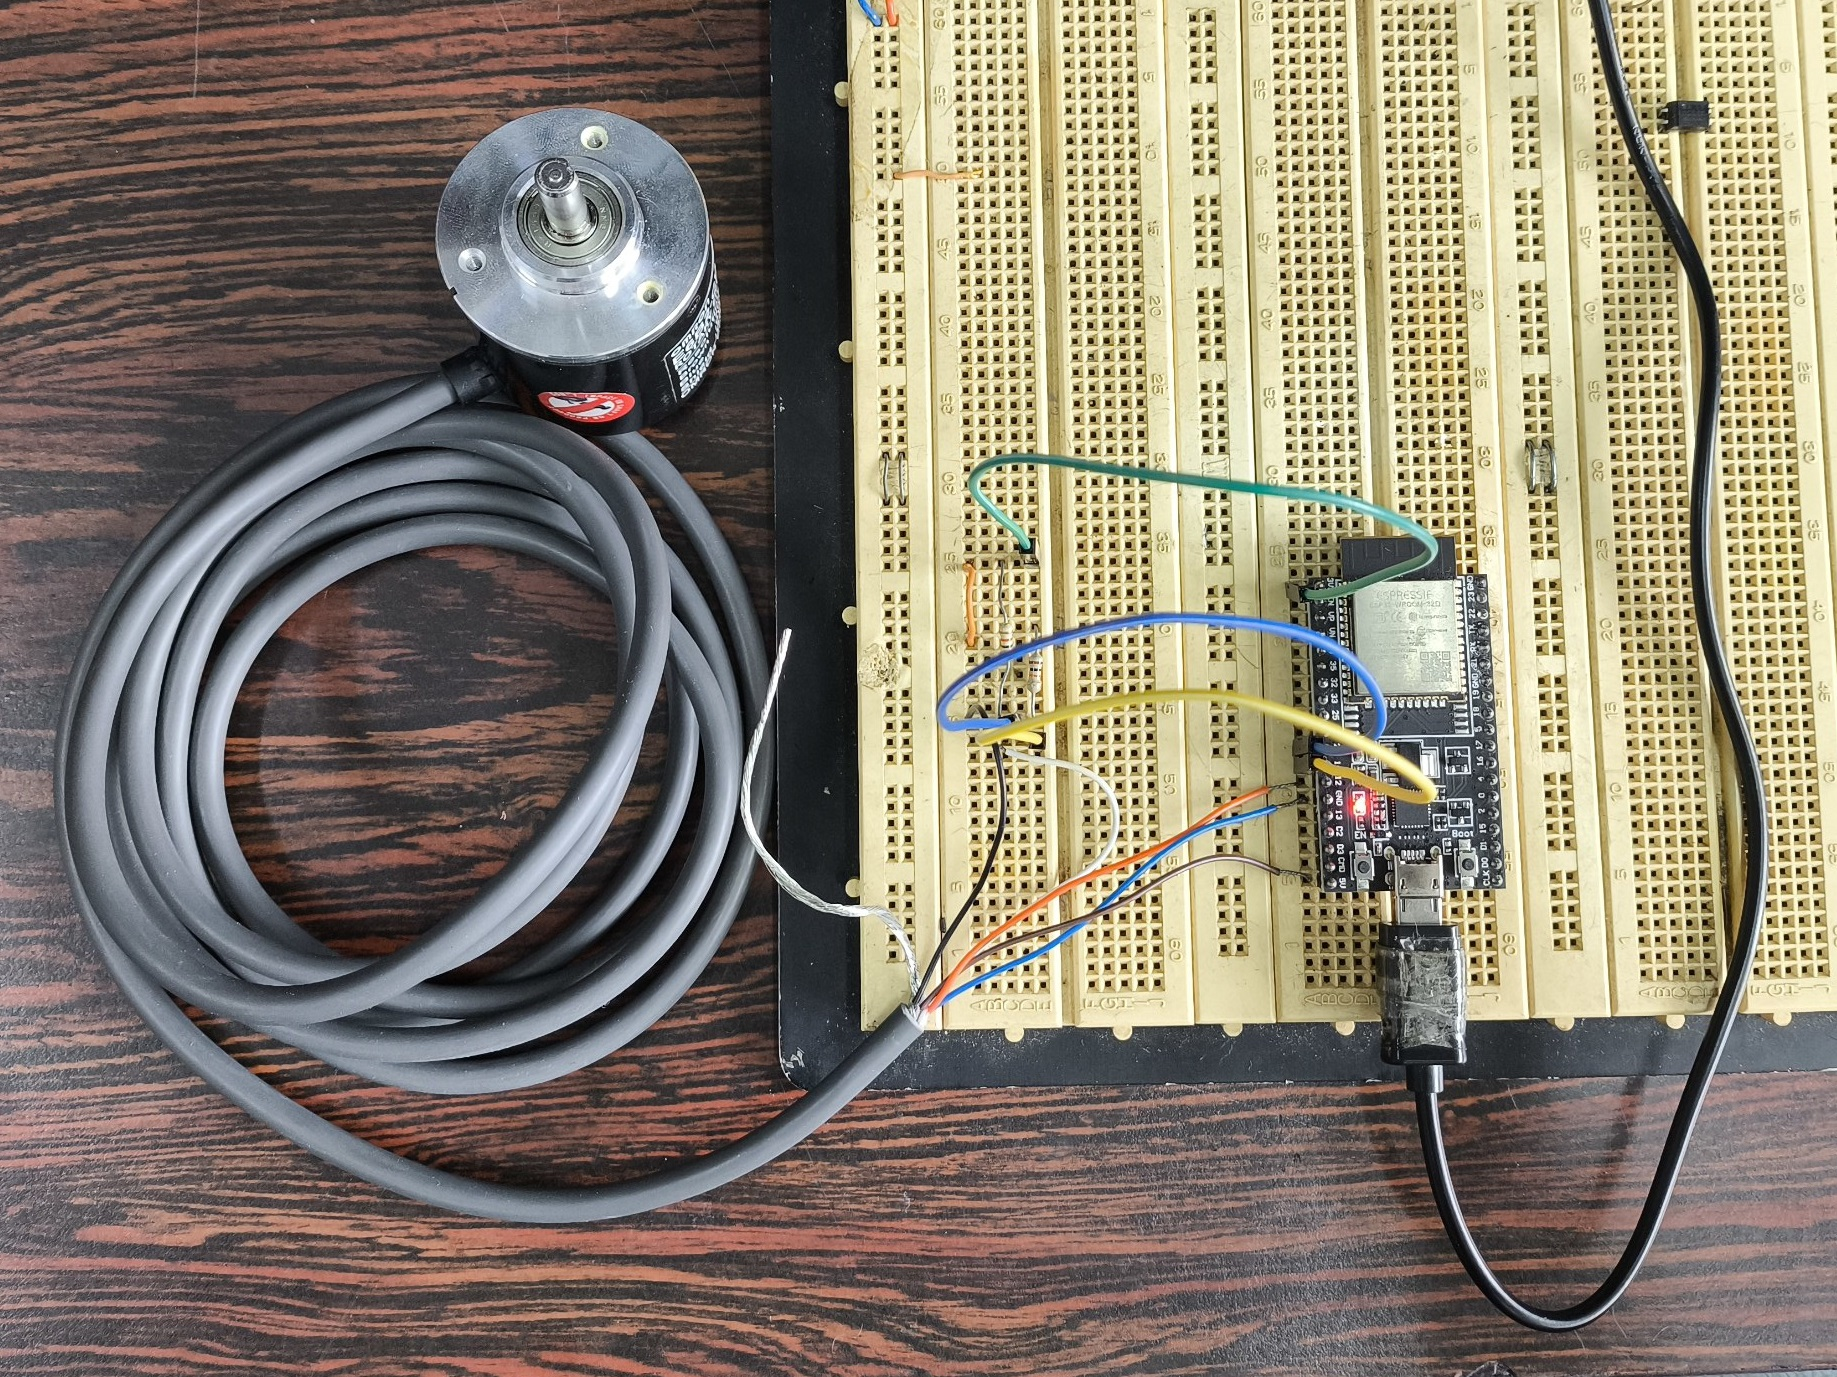
\includegraphics[width=\textwidth]{fig/encoder-esp.jpg}
                \caption{Montaje mínimo para el funcionamiento del encoder y lectura a través del esp32.}
            \end{figure}
        }
        \column{0.5\textwidth}{
            El firmware del ESP32, usando el periférico PCNT, interpreta las señales para calcular el ángulo y detectar el pulso de la fase Z, reseteando el contador. \\
            \begin{figure}[H]
                \centering
                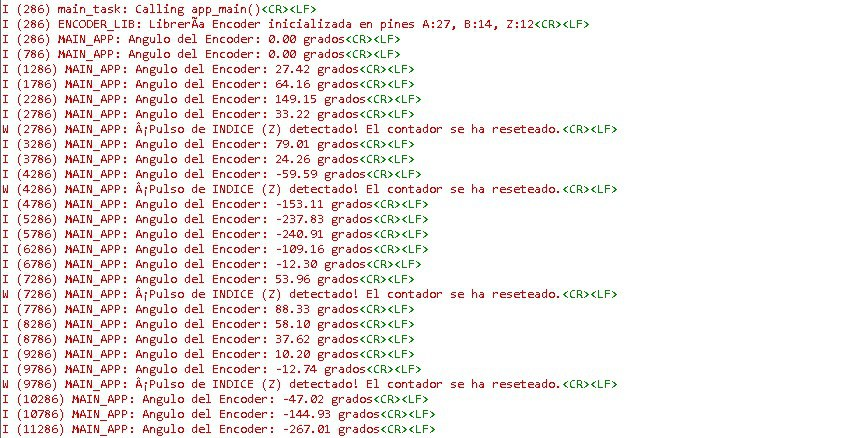
\includegraphics[width=\textwidth]{fig/encoder-code.jpg}
                \caption{Salida serial del codigo respectivo.}
            \end{figure}
        }
    \end{columns}
\end{frame}

\section{Implementación de motor a paso.}

\begin{frame}{Librería de stepperMotor}
    \begin{columns}[c]
        \column{0.5\textwidth}{
        \begin{figure}[H]
            \centering
            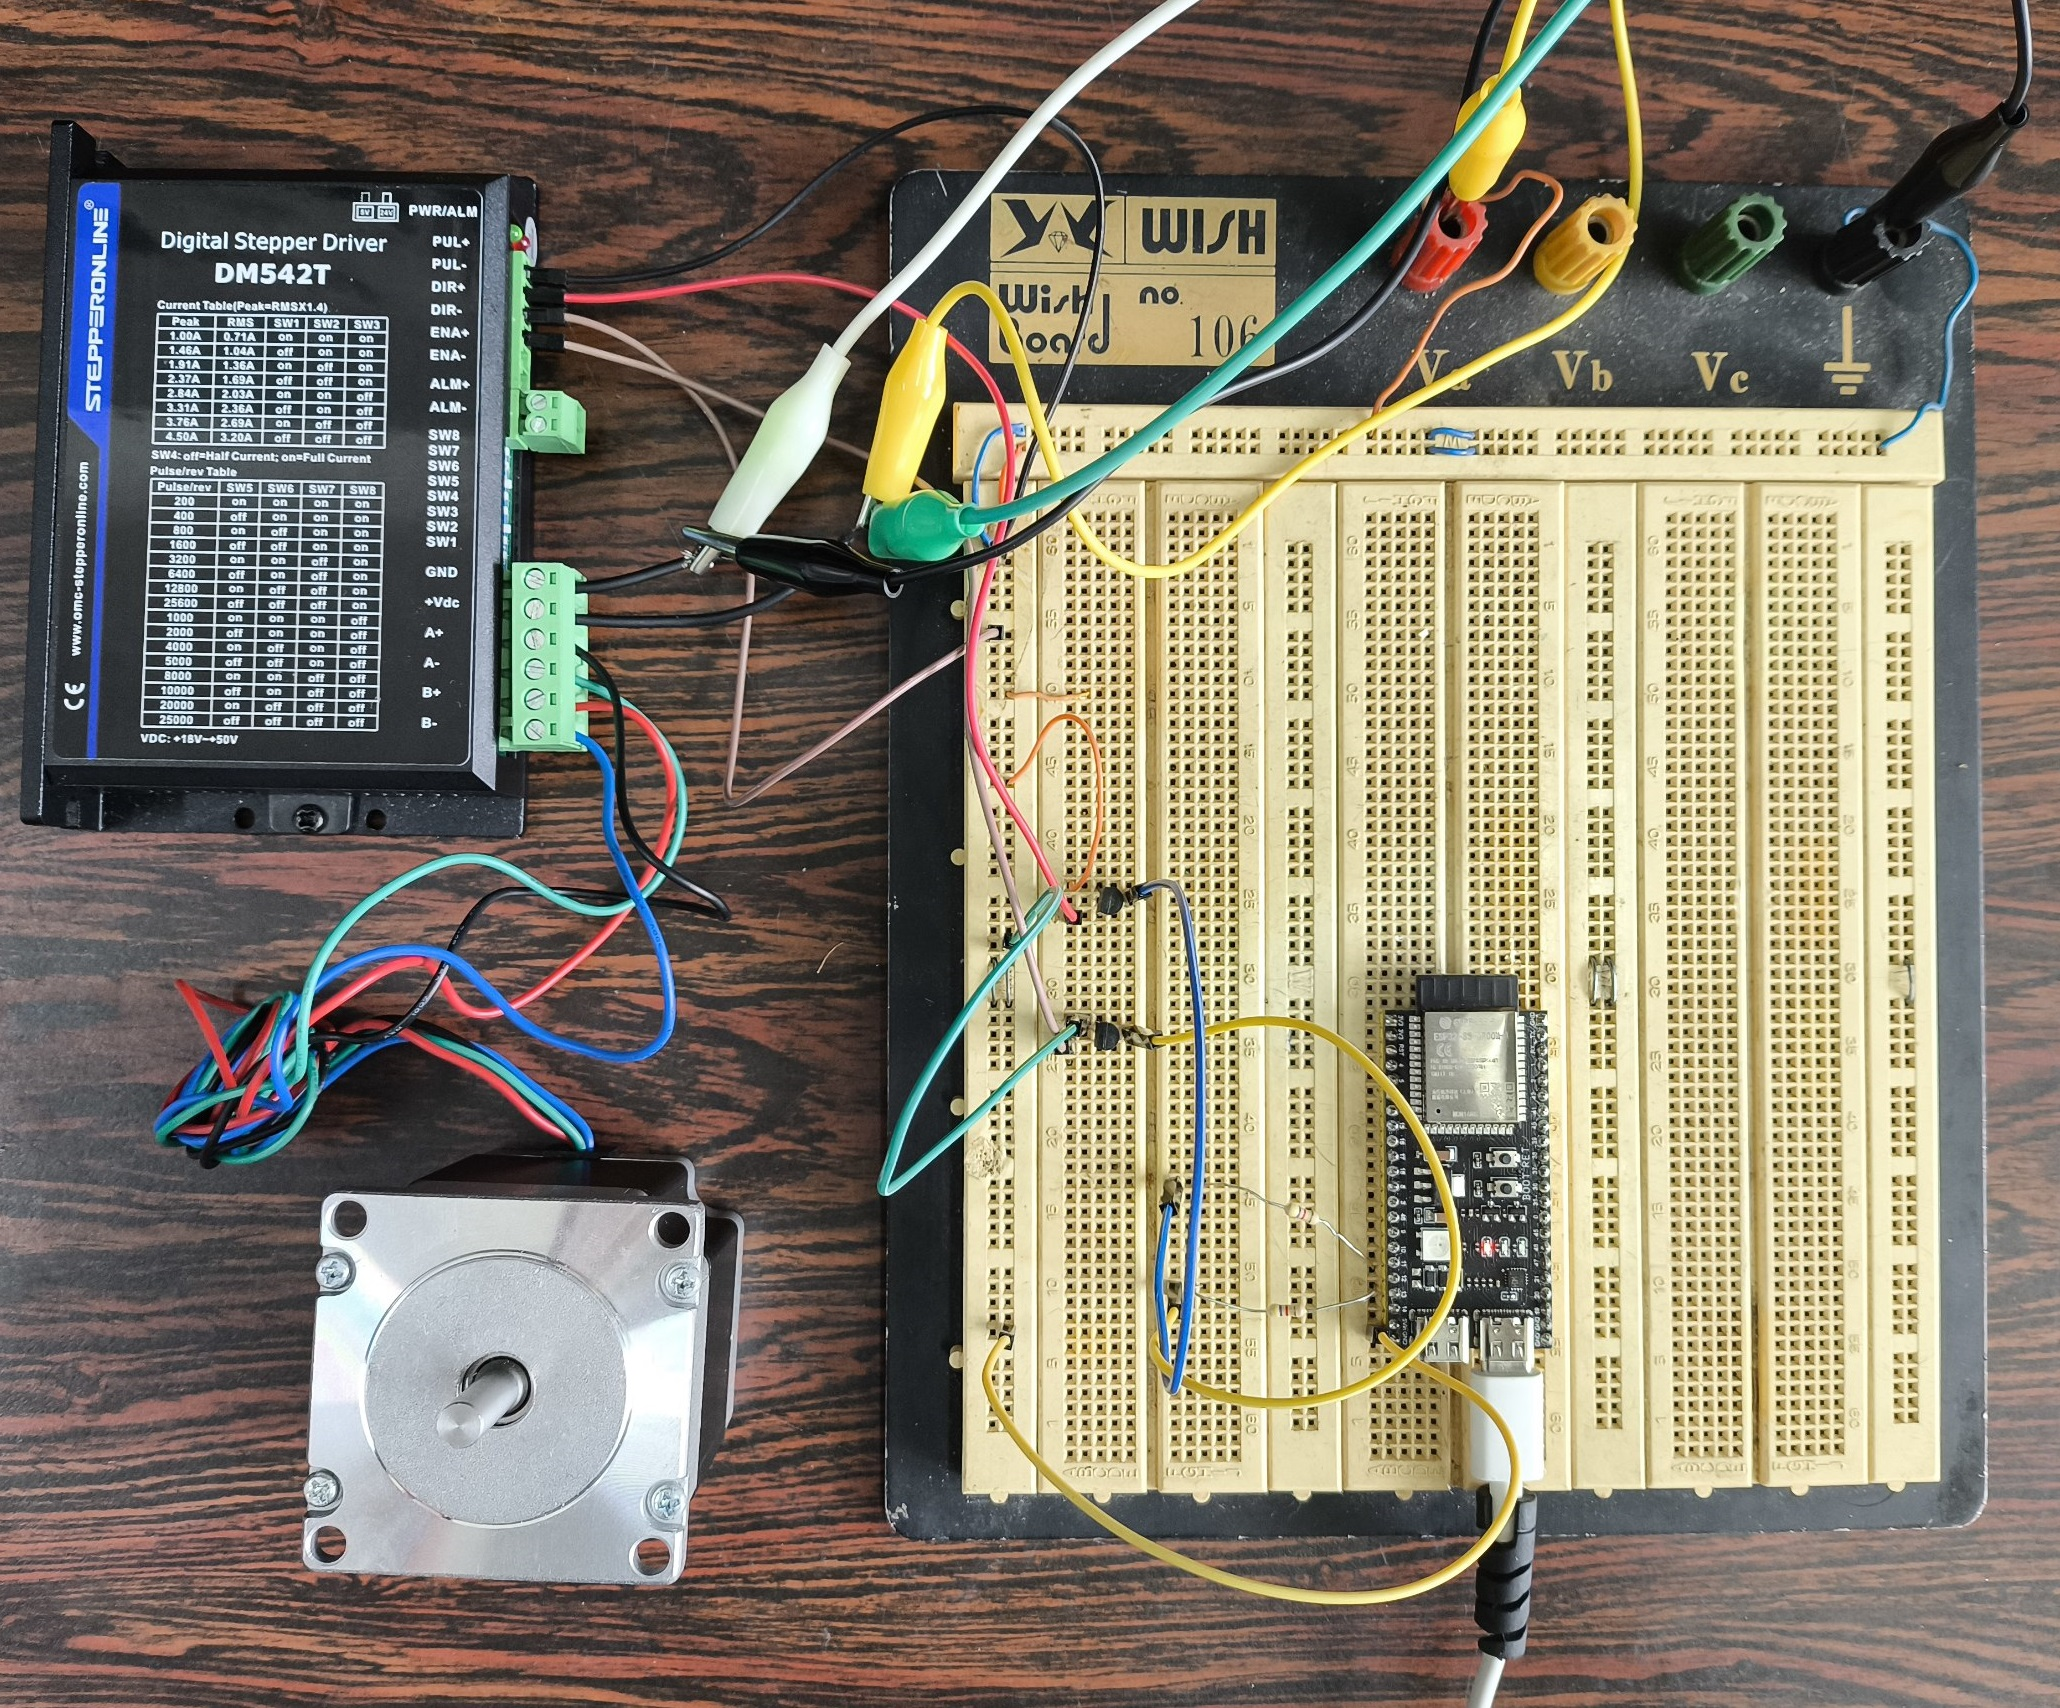
\includegraphics[width=\textwidth]{fig/motor-esp.jpg}
            \caption{Diagrama de conexiones driver y motor, en conjunto con el ESP32.}
        \end{figure}
        }

        \column{0.5\textwidth}{
            \begin{exampleblock}{Fórmula General:}
                \begin{equation}\label{eq:f}
                    \frac{f_{pulsos}}{f_{motor}} = PPR
                \end{equation}
            \end{exampleblock}
            \begin{itemize}
                \item $f_{pulsos}$: Frecuencia de pulsos enviada al driver por PUL (Hz).
                \item $f_{motor}$: Frecuencia de rotación del motor (Hz) (RPM/60).
                \item $PPR$: Pulsos por revolución del motor que depende del driver.
            \end{itemize}          
        }
    \end{columns}  
\end{frame}

\section{Fabricación de módulo controlador.}

\begin{frame}
    \begin{columns}[c]
        \column{0.5\textwidth}{
            \begin{block}{Diseño}
                \begin{figure}[H]
                    \centering
                    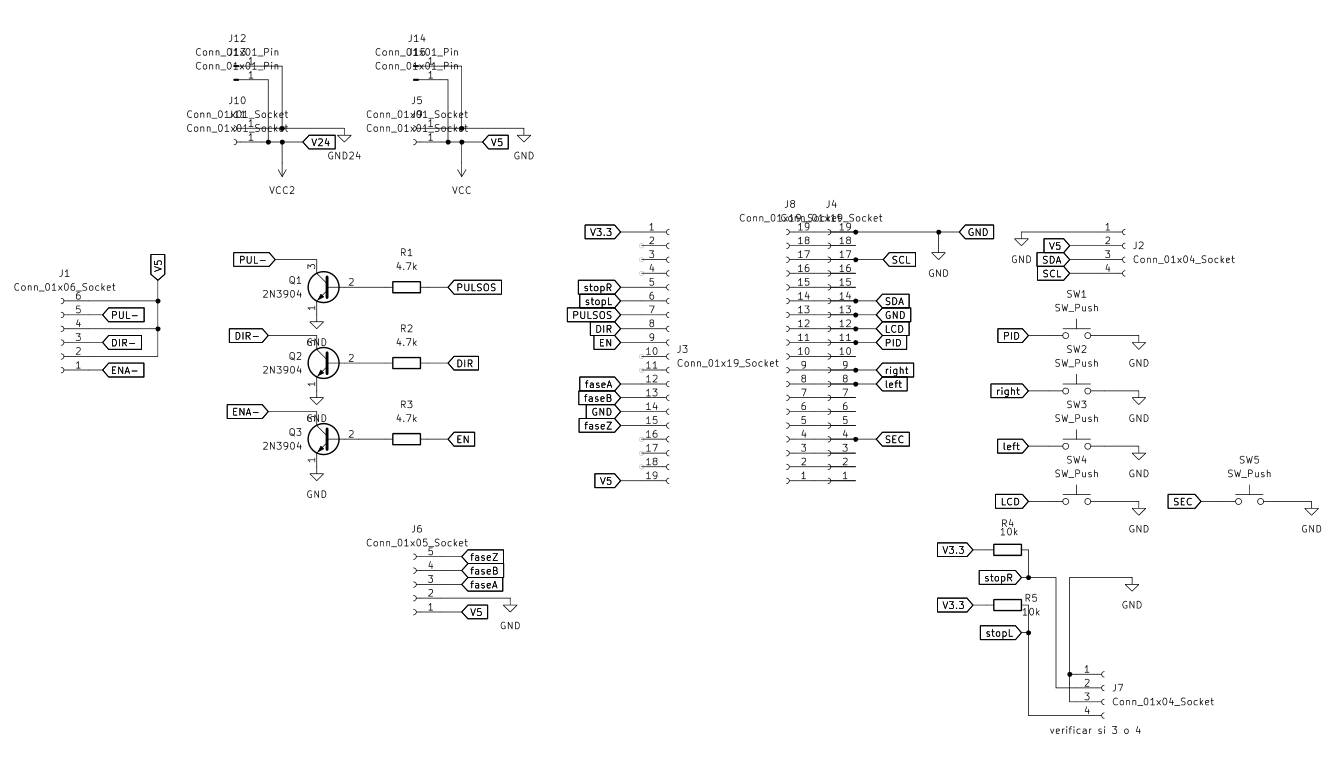
\includegraphics[height=2cm]{fig/kicad-esquematico.png}
                    \caption{Diagrama esquemático del módulo de trabajo.}
                \end{figure}
                \begin{figure}[H]
                    \centering
                    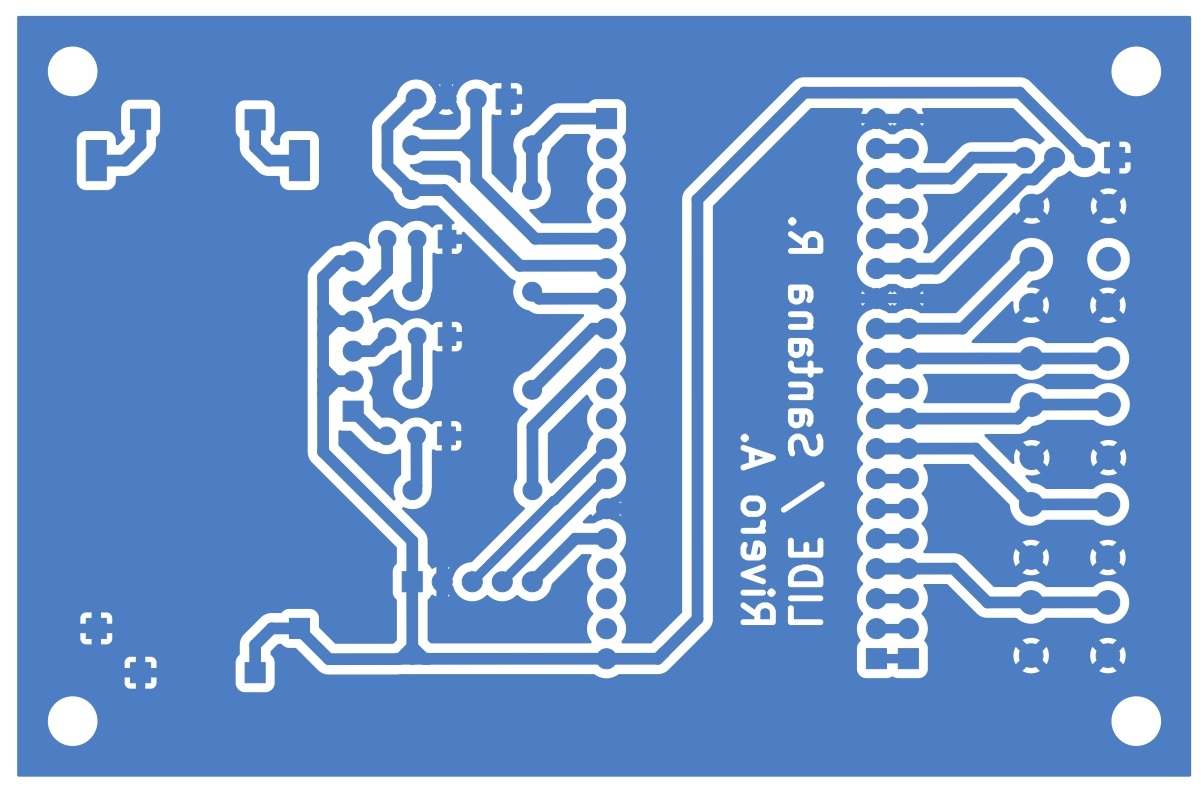
\includegraphics[height=2cm]{fig/kicad-placa.jpg}
                    \caption{Layout del módulo de trabajo.}
                \end{figure}
            \end{block}
        }
        \column{0.5\textwidth}{
            \begin{exampleblock}{Implemetación}
                \begin{figure}[H]
                    \centering
                    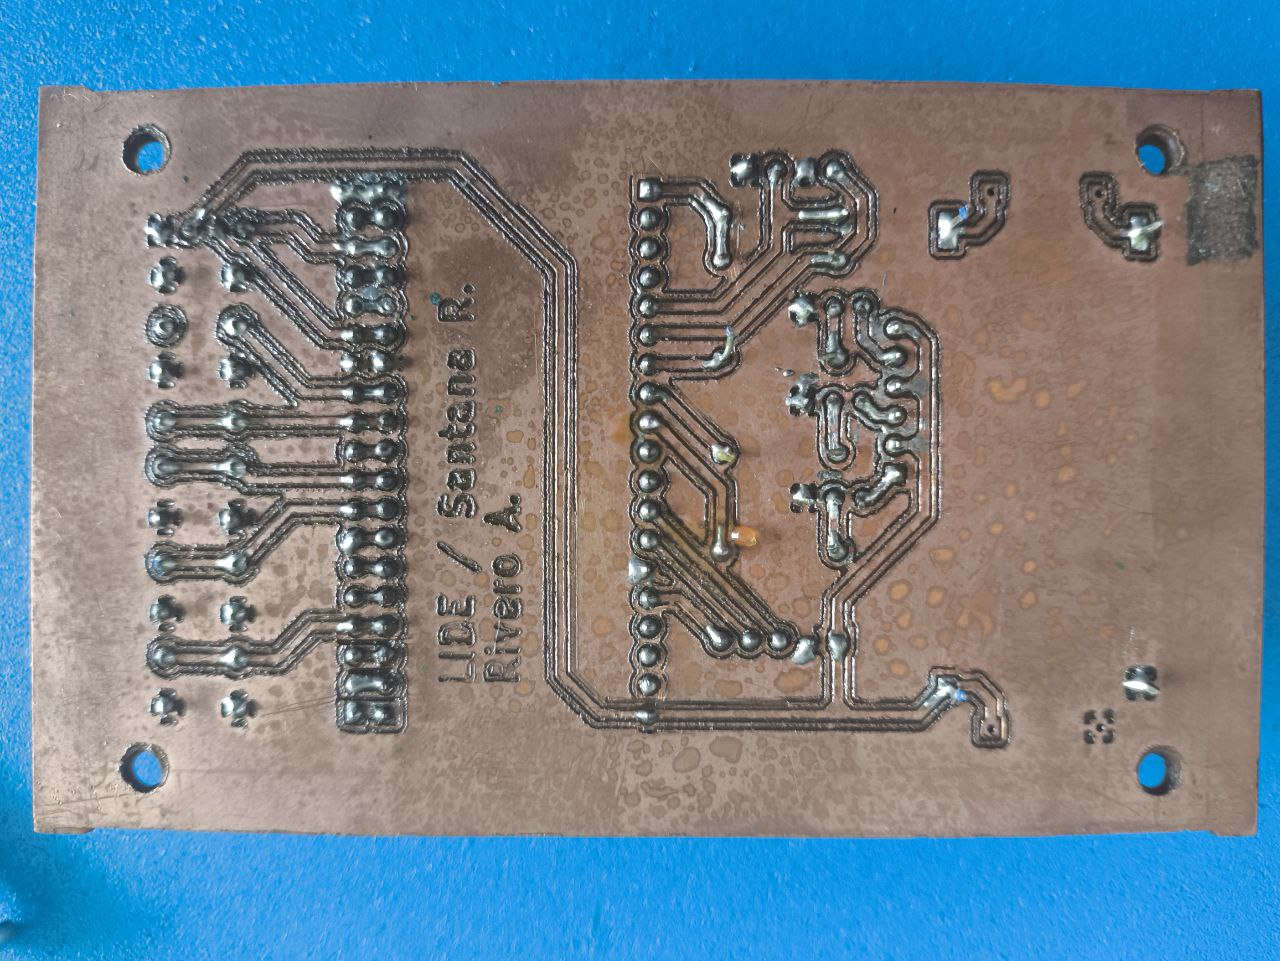
\includegraphics[height=2cm]{fig/placaB.jpg}
                    \caption{Vista inferior de modulo de trabajo basado en esp32.}
                \end{figure}
                \begin{figure}[H]
                    \centering
                    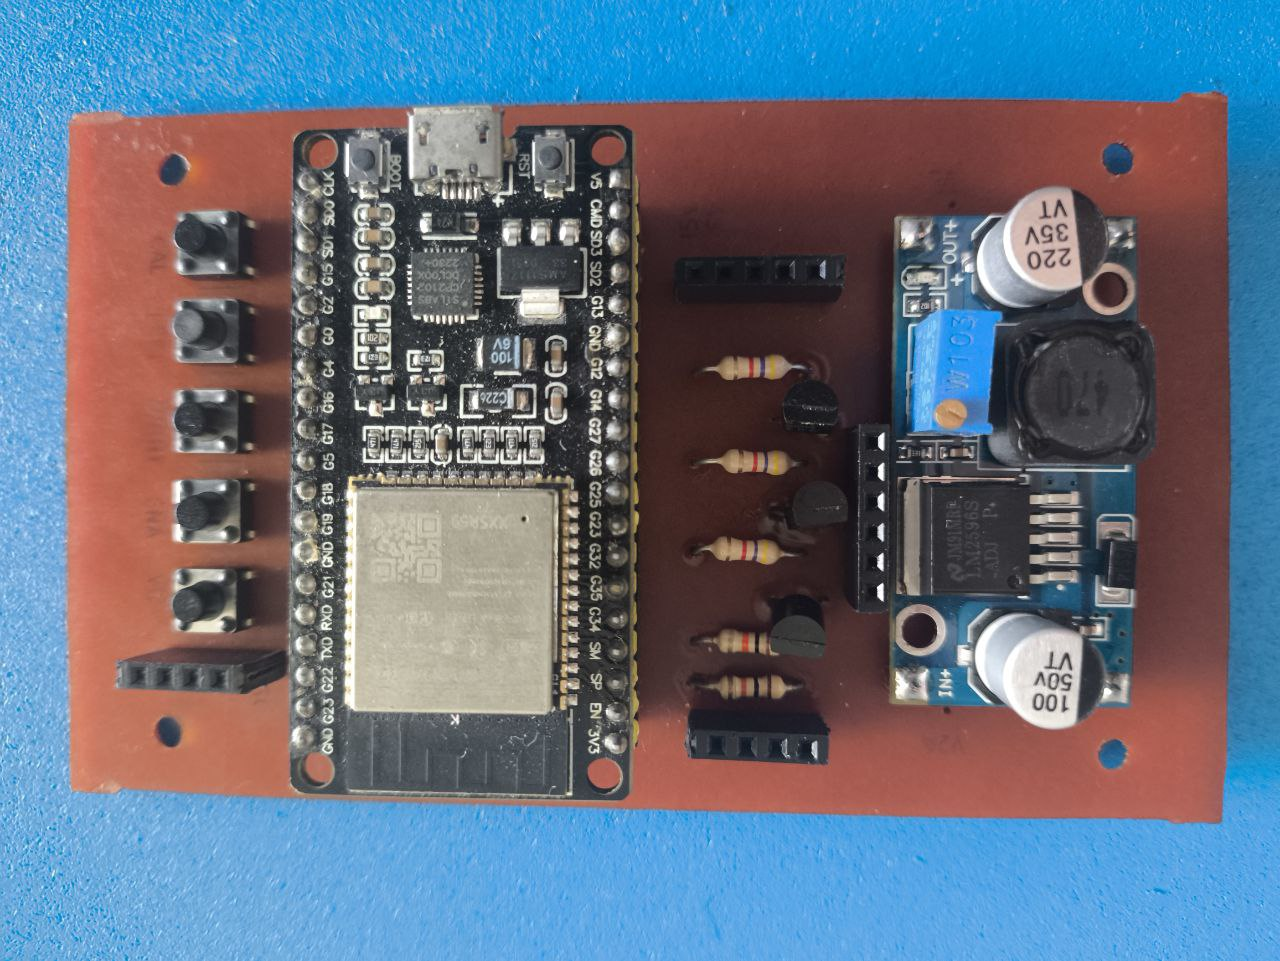
\includegraphics[height=2cm]{fig/placaF.jpg}
                    \caption{Vista superior de modulo de trabajo basado en esp32.}
                \end{figure}
            \end{exampleblock}
        }
    \end{columns}
\end{frame}

\section{Integración y funcionamiento.}

\begin{frame}{Conexiones utilizadas}

    Los códigos implementados en el ESP32 se encuentran en el repositorio de GitHub citado en \cite{Santana2025GitHub}, donde se indican las tres librerias principales \textbf{"lib\_encoder"}, \textbf{"lib\_stepperMotor"} y \textbf{"lib\_LCD"}.
    
    \begin{columns}[c]
        \column{0.5\textwidth}
            \begin{block}{Encoder}
                \begin{figure}[H]
                    \centering
                    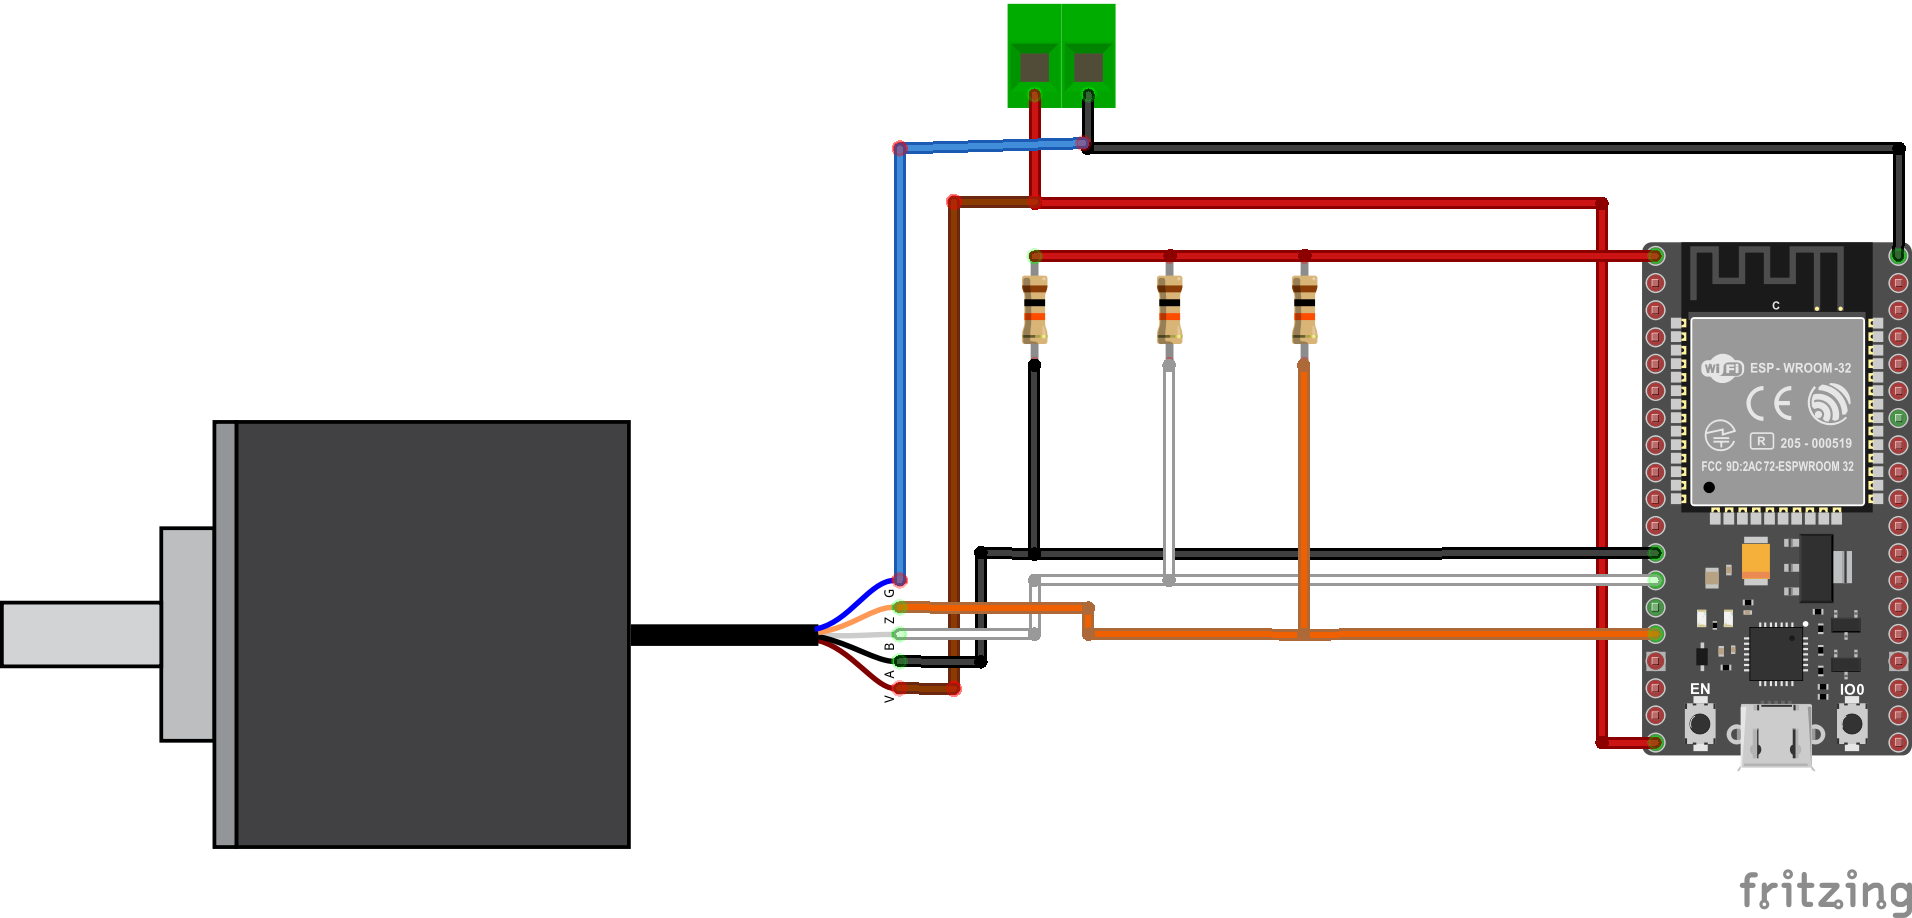
\includegraphics[width=\textwidth]{fig/diagrama_conexion_encoder_bb.png}
                    \caption{Diagrama de conexiones de integración encoder y esp32.}
                \end{figure}
            \end{block}
        
        \column{0.5\textwidth}
            \begin{exampleblock}{Motor y driver}
                \begin{figure}[H]
                    \centering
                    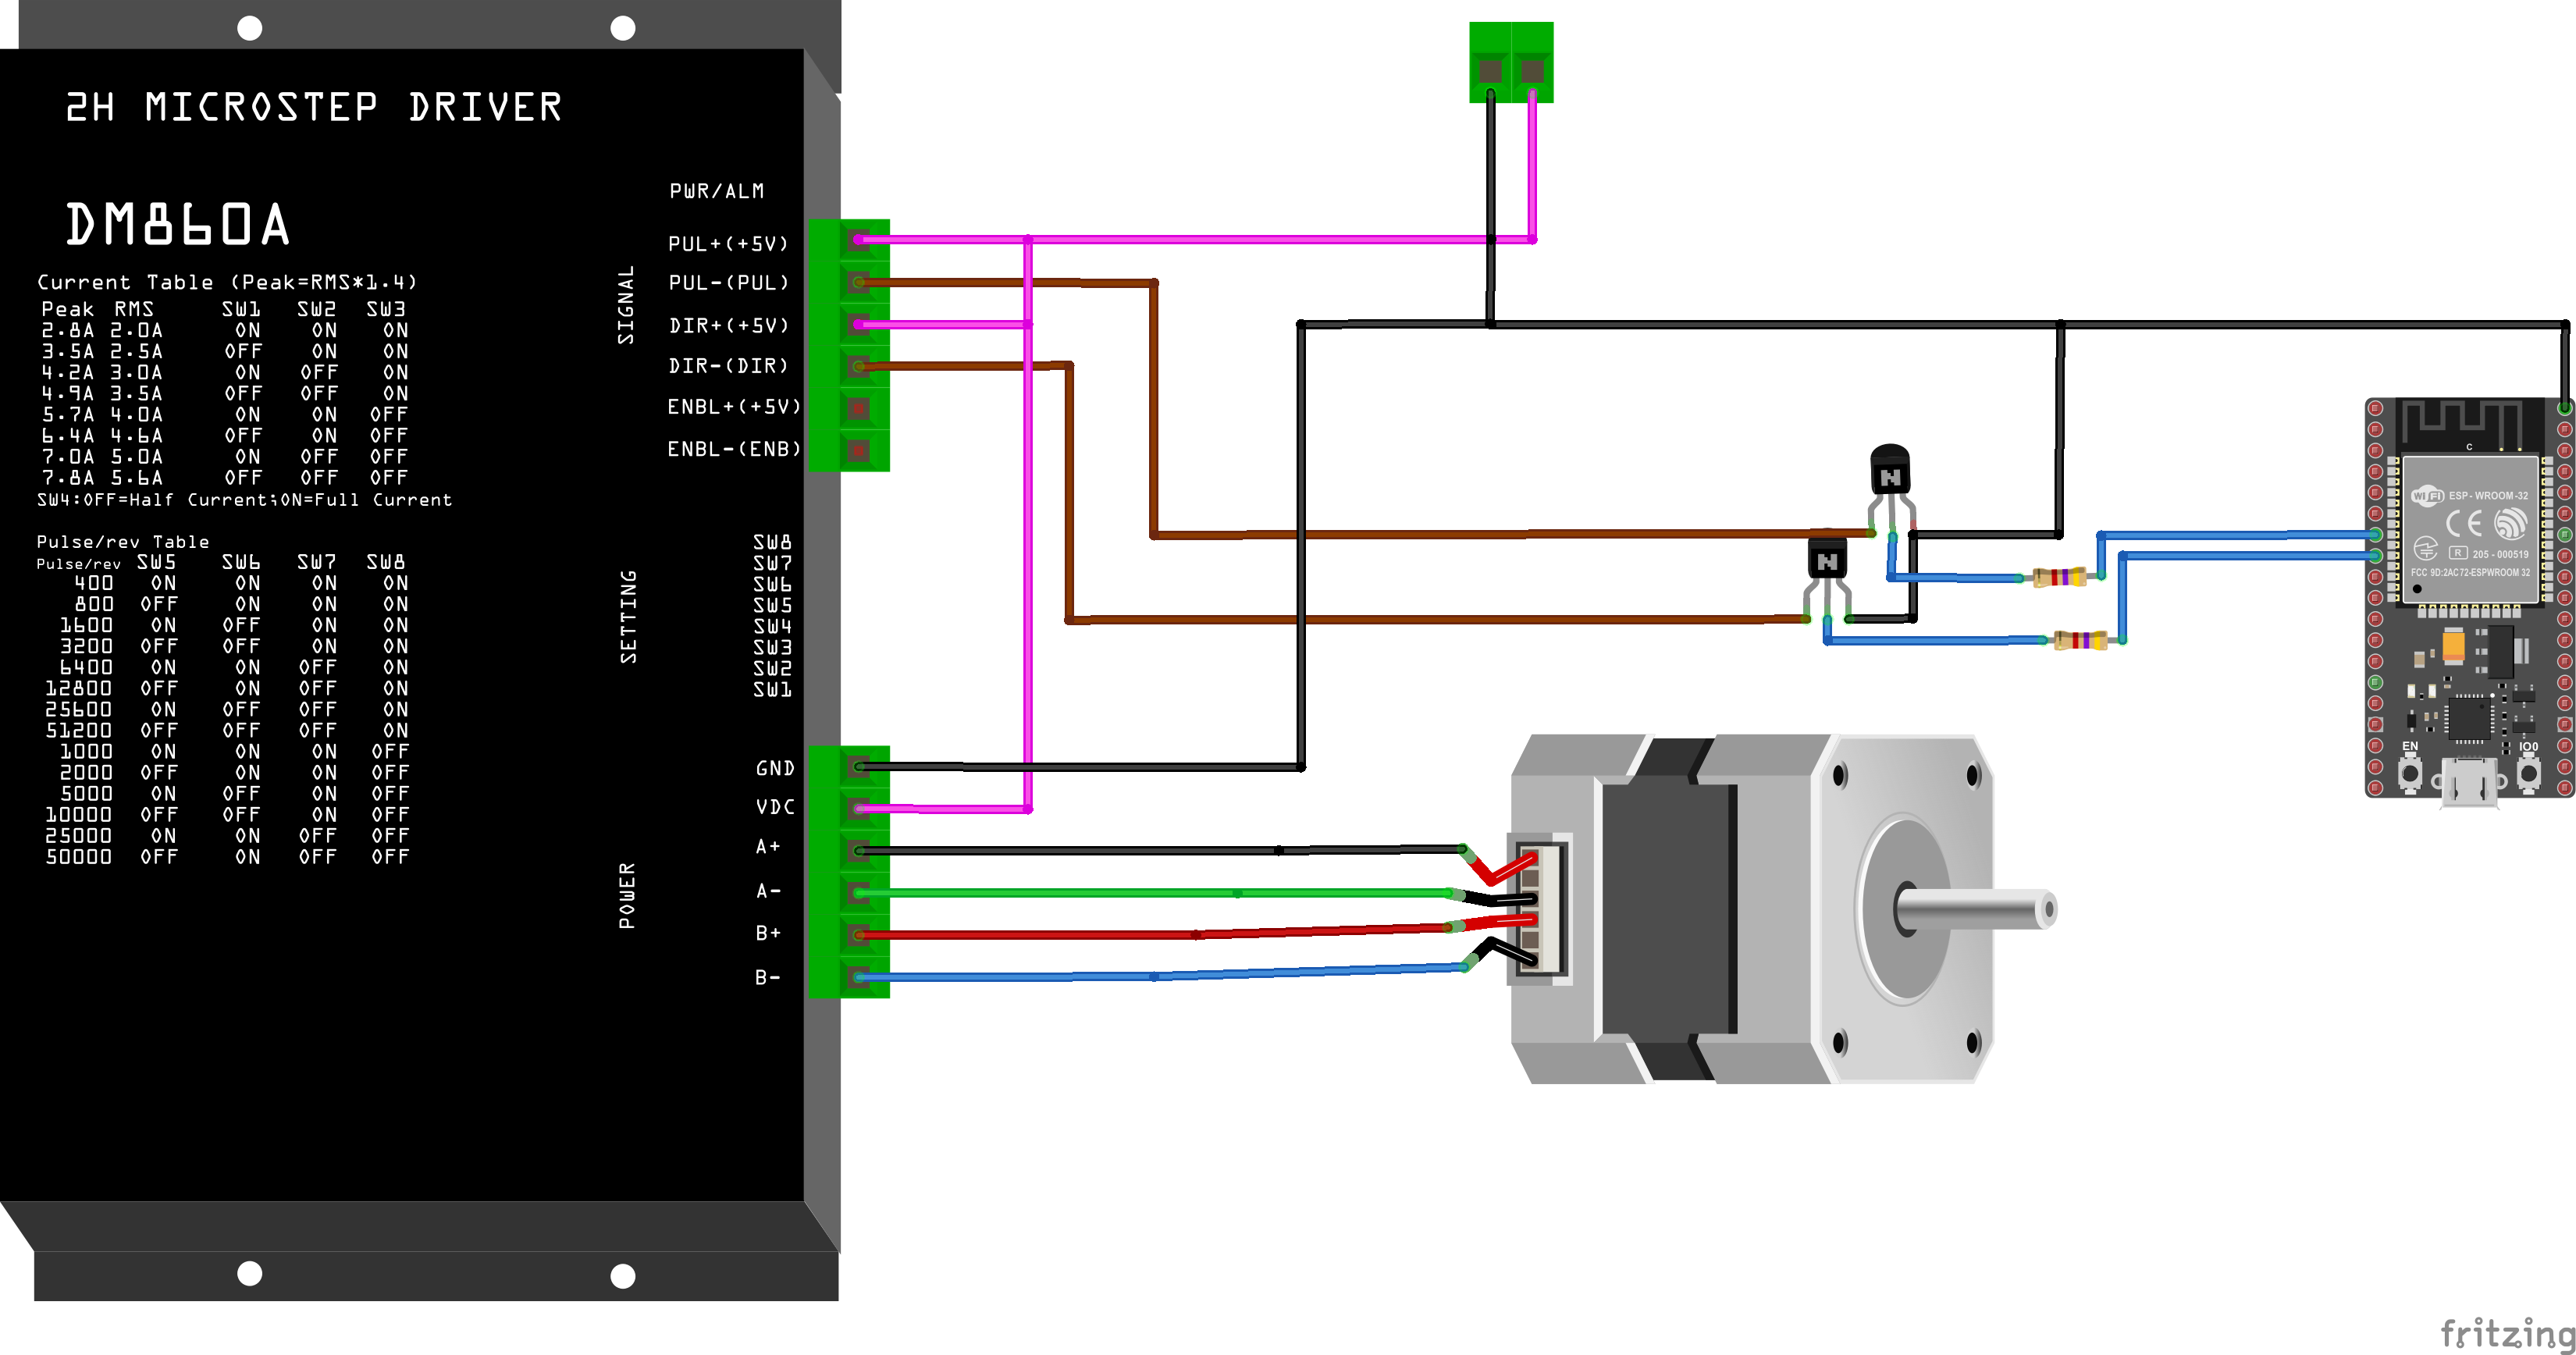
\includegraphics[width=\textwidth]{fig/diagrama_conexion_motor_bb.png}
                    \caption{Diagrama de conexiones driver y motor, en conjunto con el esp32.}
                \end{figure}
            \end{exampleblock}
              
    \end{columns}

\end{frame}

\begin{frame}{Diagrama de conexiones del sistema integrado.}

    \begin{figure}[H]
        \centering
        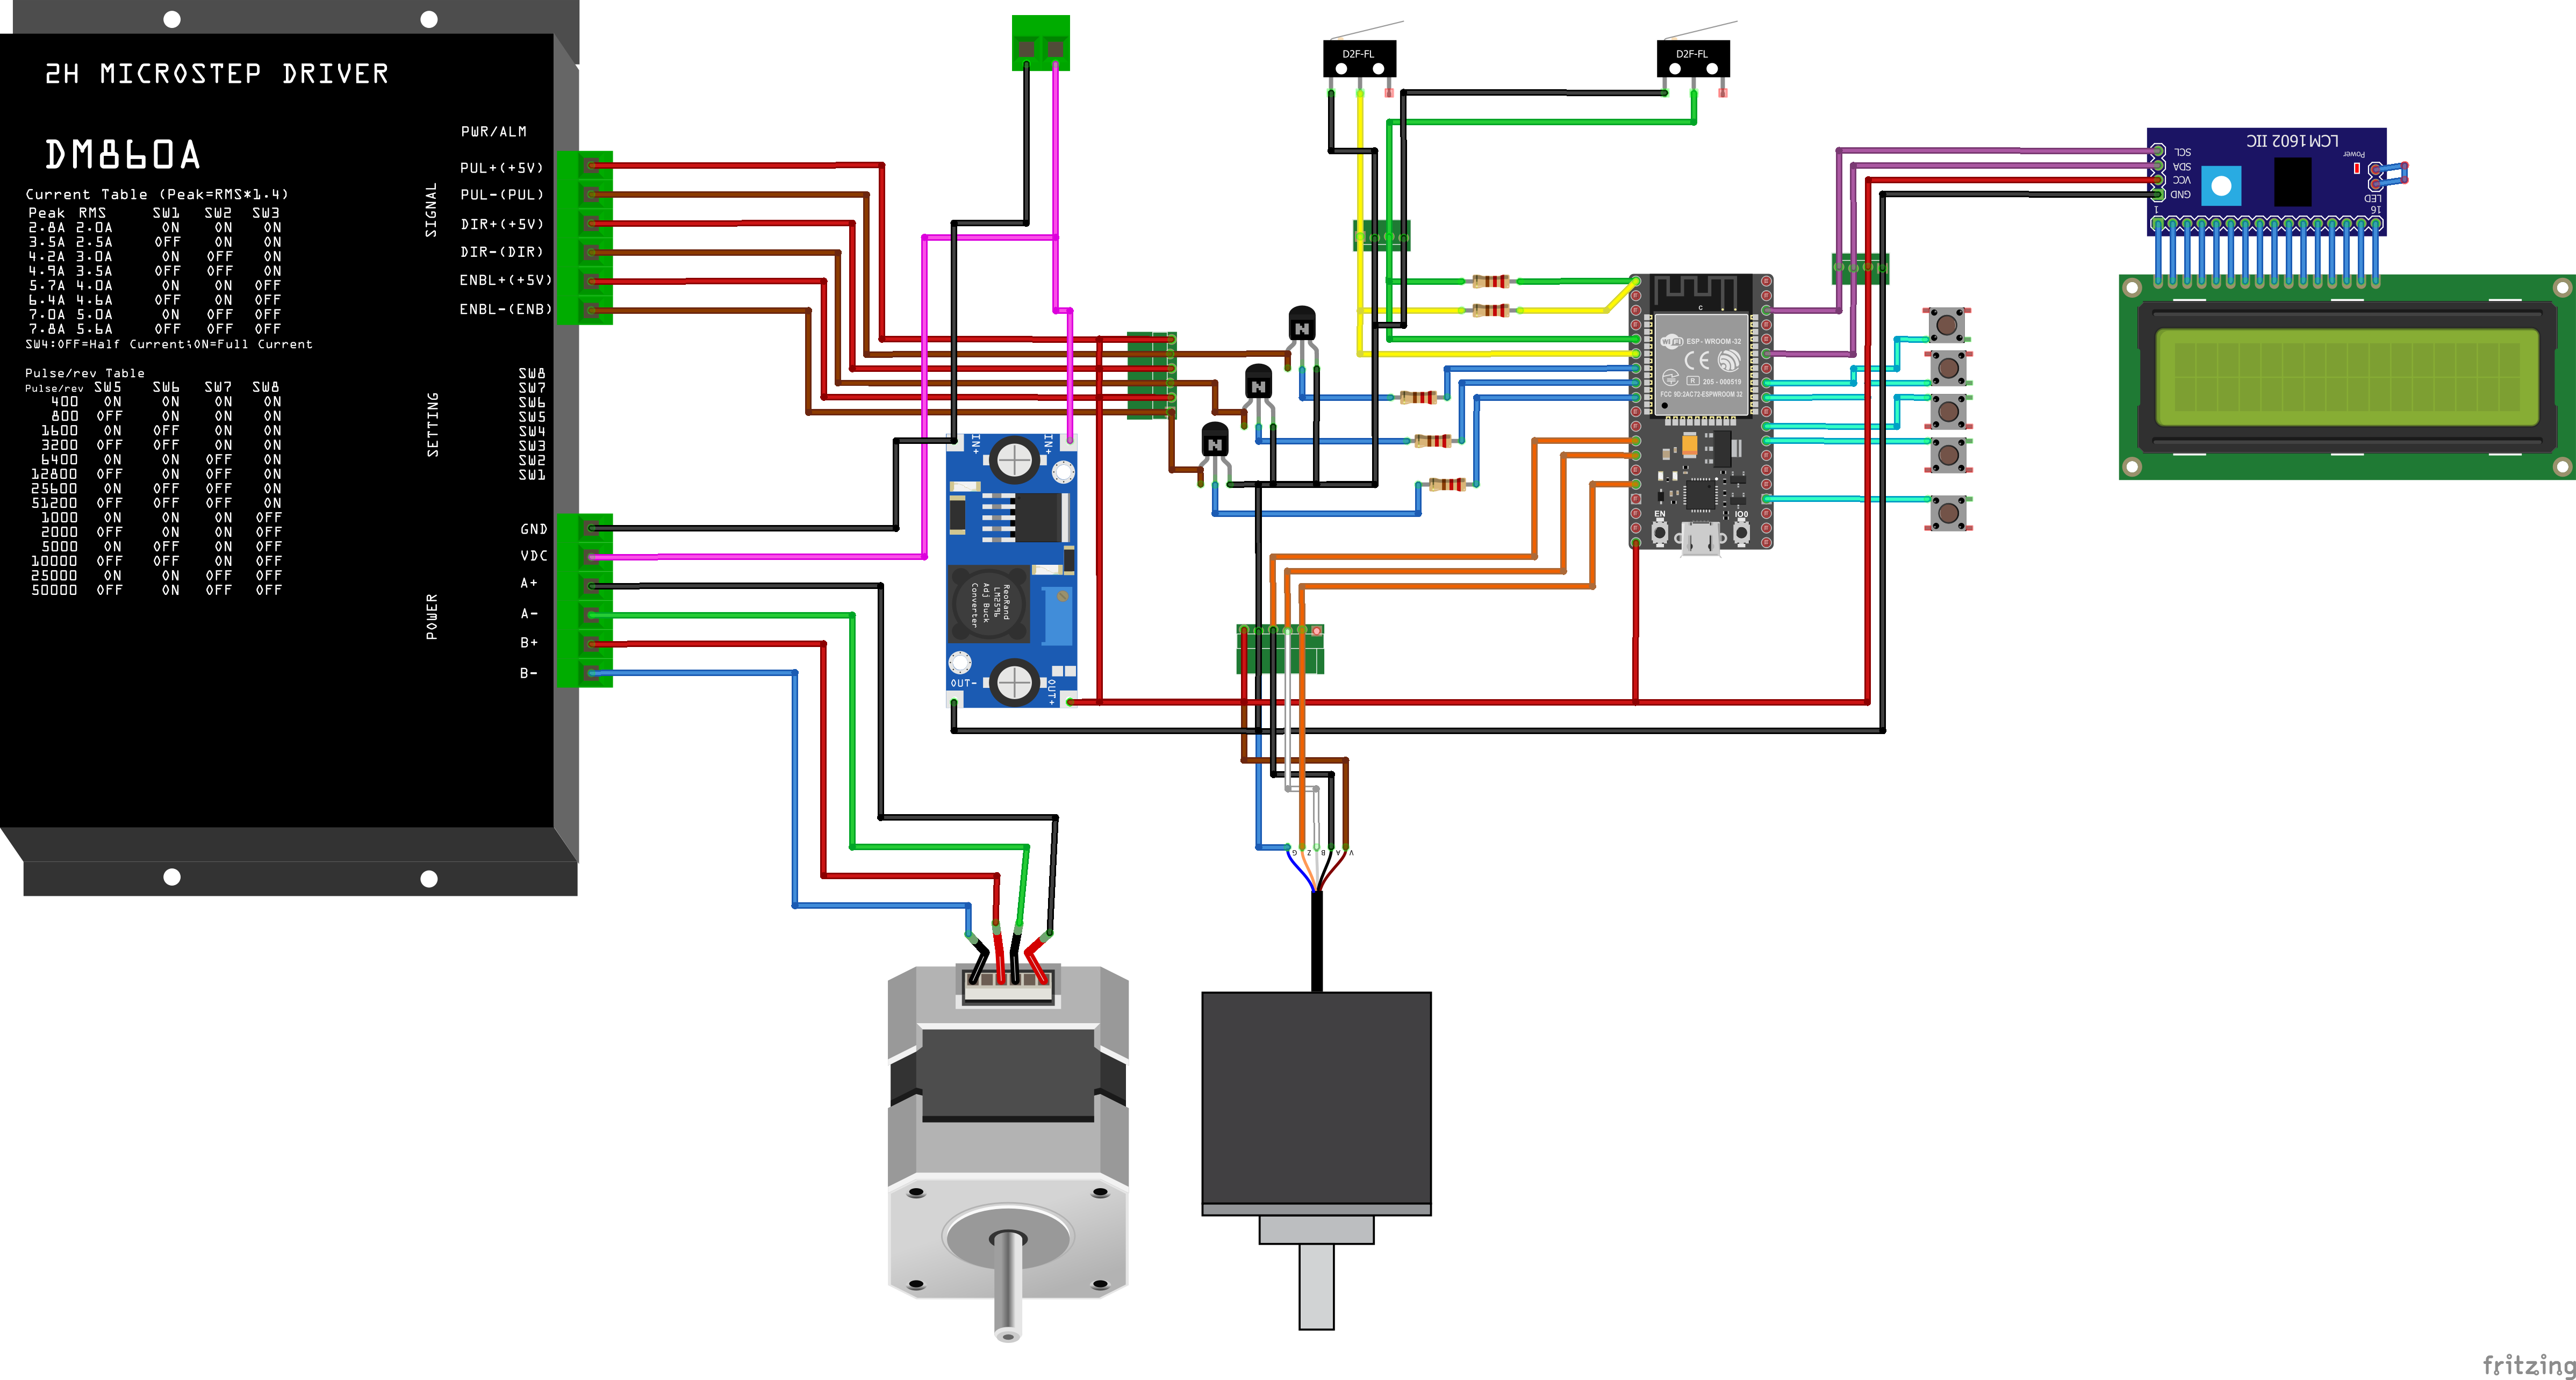
\includegraphics[width=0.9\textwidth]{fig/diagrama_conexion_control_bb.png}
        %\caption{Diagrama de conexiones de sistema.}
    \end{figure}

\end{frame}

\section{Referencias Bibliográficas}

\begin{frame}{Referencias}%[allowframebreaks]
    \nocite{*}
    \printbibliography
\end{frame}

\begin{frame}[plain]
    \itmofondo{itmo/fondoelectro.jpg}{
    \vfill
    \Huge{¡Gracias!}
    \vfill
    }
\end{frame}

\end{document}
